\noindent
El temario se dividirá principalmente en tres bloques. El primer capítulo se corresponde con una breve introducción de ciertas herramientas necesarias para los otros tres. A partir del segundo comienza la susodicha división en bloques, cada uno de ellos correspondiente con un parcial de la asignatura.
El segundo capítulo se corresponde con el primer bloque, de transporte. El tercero con el segundo bloque, de mecánica de fluidos. Por último, el cuarto con el tercer bloque, relacionado con modelos en el ámbito de la biología.\newpage

\chapter{Introducción. Recordatorios}
\noindent

\section{Gradiente}

Consideramos $N \in \N$ fijo y $f : \R^N \to \R$ (campo escalar), así como $x = (x_1, \ldots, x_N) \in \R^N$. El gradiente 
recordemos que se define como $$\nabla f (x) = \left( \dfrac{\partial f}{\partial x_1}, \ldots, 
\dfrac{\partial f}{\partial x_N} \right)(x) \quad \text{\underline{VECTOR}}$$
Este vector nos indica la dirección de máximo cambio.

\begin{proof}
    Basta considerar $v \in \R^N, |v| = 1$. Recordando que $$D_vf = \langle \nabla f(x), v \rangle = |\nabla f(x)| 
    \overbrace{|v|}^{1} \cos(\widehat{\nabla f(x)}{v})$$
    Para que sea máximo (escalarmente), el coseno debe ser máximo (1), es decir, el ángulo entre el gradiente y 
    $v$ debe ser 0, por lo que el gradiente y $v$ son vectores paralelos, o sea, tienen la misma dirección.
    Por lo tanto, necesariamente\footnote{Suponiendo que $\nabla f(x) \neq 0$.}
    $$v = \dfrac{\nabla f(x)}{|\nabla f(x)|}$$
    y por definición de $v$, este tiene la dirección de máximo cambio.
\end{proof}

    Si consideramos un campo vectorial, $f: \R^N \to \R^N$, podemos considerar el jacobiano componente a componente. Así, si
    $f = (f_1, \ldots, f_N)$, tenemos que 
    $$\nabla f = \begin{pmatrix} 
        \dfrac{\partial f_1}{\partial x_1} & \cdots & \dfrac{\partial f_1}{\partial x_N} \\ 
        \vdots & \ddots & \vdots \\ 
        \dfrac{\partial f_N}{\partial x_1} & \cdots & \dfrac{\partial f_N}{\partial x_N} 
    \end{pmatrix} = J[f] \quad \text{\underline{MATRIZ JACOBIANA}}$$ 

\newpage

\section{Divergencia}\label{section:div}

\subsection{Motivación del concepto}

Supongamos que tenemos un fluido (líquido, por ejemplo, agua). Nos queremos fijar en una partícula (concreta pero arbitraria) 
del fluido, con la hipótesis de que dicho fluido se mueve en el tiempo. \\

Consideramos $u = (u_1, u_2, u_3)$, que será el campo de velocidades del fluido, a su vez supuesto conocido. Tenemos
$u = u(t,x)$, donde $t$ es la variable temporal y $q(t)$ es la posición de la partícula en el instante $t$. 
La situación queda representada en la Figura \ref{fig:f11}:

\begin{figure}[H]
    \begin{center}
        \tikzset{every picture/.style={line width=0.75pt}} %set default line width to 0.75pt        
        \begin{tikzpicture}[x=0.75pt,y=0.75pt,yscale=-1,xscale=1]
        %uncomment if require: \path (0,300); %set diagram left start at 0, and has height of 300

        %Shape: Circle [id:dp9868303673861135] 
        \draw  [fill={rgb, 255:red, 0; green, 0; blue, 0 }  ,fill opacity=1 ] (97.67,109.83) .. controls (97.67,108.45) and (98.79,107.33) .. (100.17,107.33) .. controls (101.55,107.33) and (102.67,108.45) .. (102.67,109.83) .. controls (102.67,111.21) and (101.55,112.33) .. (100.17,112.33) .. controls (98.79,112.33) and (97.67,111.21) .. (97.67,109.83) -- cycle ;
        %Curve Lines [id:da7650198021214434] 
        \draw    (100.17,109.83) .. controls (113,100.21) and (152.47,115.47) .. (144.33,87) .. controls (136.32,58.96) and (160.26,79.04) .. (187.74,61.18) ;
        \draw [shift={(189,60.33)}, rotate = 145.38] [color={rgb, 255:red, 0; green, 0; blue, 0 }  ][line width=0.75]    (10.93,-3.29) .. controls (6.95,-1.4) and (3.31,-0.3) .. (0,0) .. controls (3.31,0.3) and (6.95,1.4) .. (10.93,3.29)   ;
        %Shape: Circle [id:dp5572905211482128] 
        \draw  [fill={rgb, 255:red, 0; green, 0; blue, 0 }  ,fill opacity=1 ] (187.67,59.83) .. controls (187.67,58.45) and (188.79,57.33) .. (190.17,57.33) .. controls (191.55,57.33) and (192.67,58.45) .. (192.67,59.83) .. controls (192.67,61.21) and (191.55,62.33) .. (190.17,62.33) .. controls (188.79,62.33) and (187.67,61.21) .. (187.67,59.83) -- cycle ;

        % Text Node
        \draw (142.67,131.67) node   [align=left] {\begin{minipage}[lt]{68pt}\setlength\topsep{0pt}
        $\displaystyle q$
        \end{minipage}};
        % Text Node
        \draw (246,65.67) node   [align=left] {\begin{minipage}[lt]{68pt}\setlength\topsep{0pt}
        $\displaystyle q( t)$
        \end{minipage}};
        \end{tikzpicture}
    \end{center}
    \caption{Posición inicial e instantánea en el instante $t$}
    \label{fig:f11}
\end{figure}

La ley que nos describe este movimiento es el siguiente PVI\footnote{Para simplificar la notación, en lo que sigue escribiremos $u(q(t))\equiv u(t,q(t))$, 
entendiendo que la primera variable de $u$ es siempre el tiempo $t$.}

\begin{equation}\label{eq:ec1}
    \begin{cases}
        q'(t) = u(q(t)) \\
        q(0) = q
    \end{cases}
\end{equation}

Es decir, si conocemos el campo de velocidades, podemos escribir la ecuación, resolverla, y obtener la función $q(t)$
que nos describe el susodicho movimiento de la partícula. \\

Ahora consideramos la misma situación inicial, y queremos estudiar cómo cambia un volumen infinitesimal.
El tamaño de cada arista será $\varepsilon$, y queremos ver cómo se deforma el volumen del cubo con el tiempo.
Cuando podamos escribir dicha ecuación aparecerá de forma natural el concepto de divergencia. Las longitudes $a_q^i$, con
$i \in \{1,2,3\}$, son funciones que dependen del tiempo, pero que coinciden en el instante inicial. La situación en que nos 
encontramos viene ilustrada en la Figura \ref{fig:f12}:

\begin{figure}[H]
    \begin{center}

    \tikzset{every picture/.style={line width=0.75pt}} %set default line width to 0.75pt        

    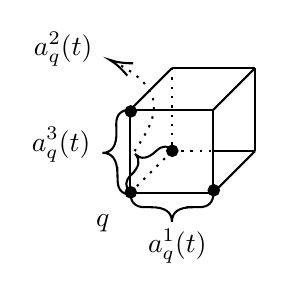
\begin{tikzpicture}[x=0.75pt,y=0.75pt,yscale=-1,xscale=1]
    %uncomment if require: \path (0,300); %set diagram left start at 0, and has height of 300

    %Shape: Circle [id:dp9868303673861135] 
    \draw  [fill={rgb, 255:red, 0; green, 0; blue, 0 }  ,fill opacity=1 ] (207.67,99.83) .. controls (207.67,98.45) and (208.79,97.33) .. (210.17,97.33) .. controls (211.55,97.33) and (212.67,98.45) .. (212.67,99.83) .. controls (212.67,101.21) and (211.55,102.33) .. (210.17,102.33) .. controls (208.79,102.33) and (207.67,101.21) .. (207.67,99.83) -- cycle ;
    %Shape: Rectangle [id:dp8440612850022642] 
    \draw   (210,60) -- (250,60) -- (250,100) -- (210,100) -- cycle ;
    %Straight Lines [id:da8160136384076409] 
    \draw    (210,60) -- (230,40) ;
    %Straight Lines [id:da546497530395401] 
    \draw    (250,60) -- (270,40) ;
    %Straight Lines [id:da011934677438056873] 
    \draw    (250,100) -- (270,80) ;
    %Straight Lines [id:da28246078787903206] 
    \draw  [dash pattern={on 0.84pt off 2.51pt}]  (230,40) -- (230,80) ;
    %Straight Lines [id:da7718883113576894] 
    \draw  [dash pattern={on 0.84pt off 2.51pt}]  (230,80) -- (250,80) ;
    %Straight Lines [id:da7573142764220282] 
    \draw    (250,80) -- (270,80) ;
    %Straight Lines [id:da3645358326064383] 
    \draw    (270,40) -- (270,80) ;
    %Straight Lines [id:da04533787187694238] 
    \draw    (230,40) -- (270,40) ;
    %Straight Lines [id:da31951741461037897] 
    \draw  [dash pattern={on 0.84pt off 2.51pt}]  (210,100) -- (230,80) ;
    %Shape: Brace [id:dp616787207683195] 
    \draw   (210,100) .. controls (210,104.67) and (212.33,107) .. (217,107) -- (220,107) .. controls (226.67,107) and (230,109.33) .. (230,114) .. controls (230,109.33) and (233.33,107) .. (240,107)(237,107) -- (243,107) .. controls (247.67,107) and (250,104.67) .. (250,100) ;
    %Shape: Brace [id:dp44451260981777607] 
    \draw   (231,80) .. controls (228.25,77.12) and (225.44,77.05) .. (222.56,79.79) -- (222.56,79.79) .. controls (218.44,83.72) and (215.01,84.24) .. (212.26,81.35) .. controls (215.01,84.24) and (214.32,87.64) .. (210.21,91.56)(212.06,89.79) -- (210.21,91.56) .. controls (207.32,94.31) and (207.25,97.12) .. (210,100) ;
    %Curve Lines [id:da7568531294421236] 
    \draw  [dash pattern={on 0.84pt off 2.51pt}]  (212,80) .. controls (220.87,66.21) and (231.67,51.45) .. (201.41,36.67) ;
    \draw [shift={(200,36)}, rotate = 25.11] [color={rgb, 255:red, 0; green, 0; blue, 0 }  ][line width=0.75]    (10.93,-3.29) .. controls (6.95,-1.4) and (3.31,-0.3) .. (0,0) .. controls (3.31,0.3) and (6.95,1.4) .. (10.93,3.29)   ;
    %Shape: Brace [id:dp9587884219726038] 
    \draw   (210,60) .. controls (205.33,60.11) and (203.06,62.5) .. (203.17,67.17) -- (203.26,70.67) .. controls (203.42,77.34) and (201.17,80.73) .. (196.51,80.84) .. controls (201.17,80.73) and (203.58,84) .. (203.75,90.67)(203.67,87.67) -- (203.83,94.17) .. controls (203.94,98.84) and (206.33,101.11) .. (211,101) ;
    %Shape: Circle [id:dp8196257583758775] 
    \draw  [fill={rgb, 255:red, 0; green, 0; blue, 0 }  ,fill opacity=1 ] (247.67,98.83) .. controls (247.67,97.45) and (248.79,96.33) .. (250.17,96.33) .. controls (251.55,96.33) and (252.67,97.45) .. (252.67,98.83) .. controls (252.67,100.21) and (251.55,101.33) .. (250.17,101.33) .. controls (248.79,101.33) and (247.67,100.21) .. (247.67,98.83) -- cycle ;
    %Shape: Circle [id:dp9899510060278905] 
    \draw  [fill={rgb, 255:red, 0; green, 0; blue, 0 }  ,fill opacity=1 ] (207.67,60.83) .. controls (207.67,59.45) and (208.79,58.33) .. (210.17,58.33) .. controls (211.55,58.33) and (212.67,59.45) .. (212.67,60.83) .. controls (212.67,62.21) and (211.55,63.33) .. (210.17,63.33) .. controls (208.79,63.33) and (207.67,62.21) .. (207.67,60.83) -- cycle ;
    %Shape: Circle [id:dp14202122866986466] 
    \draw  [fill={rgb, 255:red, 0; green, 0; blue, 0 }  ,fill opacity=1 ] (227.67,79.83) .. controls (227.67,78.45) and (228.79,77.33) .. (230.17,77.33) .. controls (231.55,77.33) and (232.67,78.45) .. (232.67,79.83) .. controls (232.67,81.21) and (231.55,82.33) .. (230.17,82.33) .. controls (228.79,82.33) and (227.67,81.21) .. (227.67,79.83) -- cycle ;

    % Text Node
    \draw (201.33,114.83) node   [align=left] {\begin{minipage}[lt]{11.79pt}\setlength\topsep{0pt}
    $\displaystyle q$
    \end{minipage}};
    % Text Node
    \draw (217,116) node [anchor=north west][inner sep=0.75pt]   [align=left] {$\displaystyle a_{q}^{1}( t)$};
    % Text Node
    \draw (162,21) node [anchor=north west][inner sep=0.75pt]   [align=left] {$\displaystyle a_{q}^{2}( t)$};
    % Text Node
    \draw (161,67) node [anchor=north west][inner sep=0.75pt]   [align=left] {$\displaystyle a_{q}^{3}( t)$};

    \end{tikzpicture}
    \end{center}
    \caption{Cubo en el instante $t$}
    \label{fig:f12}
\end{figure}

\newpage

Así, planteamos las siguientes condiciones iniciales:

$$\begin{cases}
    a_q^1(0) = (\varepsilon, 0, 0) \\
    a_q^2(0) = (0, \varepsilon, 0) \\
    a_q^3(0) = (0, 0, \varepsilon)
\end{cases}$$

Buscamos entonces describir $a_q^i(t)$, para $i \in \{1,2,3\}$. Vemos que $q(t) + a_q^i(t)$ nos da la posición
de cada uno de los vértices (para cada $i$), y dicha evolución en el tiempo la medimos con su derivada
$$(q(t) + a_q^i(t))'.$$
De aquí deducimos una ley análoga a la que teníamos antes
$$(q(t) + a_q^i(t))' = u(q(t) + a_q^i(t)).$$
Aplicando la linealidad de la derivada, obtenemos
$$q'(t) + (a_q^i)'(t) = u(q(t) + a_q^i(t))$$
y usando \eqref{eq:ec1}~llegamos a 
$$u(q(t)) + (a_q^i)'(t) = u(q(t) + a_q^i(t)).$$

Nos disponemos en este punto a realizar un desarrollo de Taylor de la función $u$ en torno a $q(t)$, es decir\footnote{Suponemos que, al menos, $u(t, \cdot) \in C^2(\R^3, \R^3)$,
es decir, para cada $t$ instante de tiempo fijo, pongamos en $\left[0, T\right[$, el campo es $C^2$ respecto de $x$.)}

$$u(q(t) + a_q^i(t)) = u(q(t)) + \nabla u (q(t)) a_q^i(t) + O(a_q^i(t)^2)$$

La matriz jacobiana de $u$ ($\nabla u$) aparece debido a que $u$ es un campo vectorial. El segundo sumando se debe a que estamos haciendo la derivada de un campo vectorial, por lo que tenemos una matriz y 
el segundo factor es un vector\footnote{Será fundamental saber con lo que estamos trabajando (matriz, vector, etc...) 
durante el curso.}, y el término de error suponemos que es lo suficientemente pequeño como para poder 
despreciarlo. \\

Juntando todo, llegamos a

$$u(q(t)) + (a_q^i)'(t) = u(q(t)) + \nabla u (q(t)) a_q^i(t) + \cancel{O(a_q^i(t)^2)},$$

por lo que simplificando el primer sumando de cada miembro de la igualdad anterior deducimos que 

$$(a_q^i)'(t) = \nabla u (q(t)) a_q^i(t)$$

Esta ecuación será fundamental para el último paso, que es estudiar cómo cambia el volumen del cubo. Llamando $Q$ al cubo,
y denotando a su volumen por $V_Q$, obtenemos\footnote{Recordando que el volumen del cubo se halla con el producto mixto.} que
$$V_Q(t) = \det(a_q^1(t), a_q^2(t), a_q^3(t)) = \begin{vmatrix}
    a_q^1(t) | a_q^2(t) | a_q^3(t) 
\end{vmatrix}.$$

Y la variación del volumen viene determinada por $V'_Q(t)$\footnote{Recordando que la derivada de un determinante se hace
por columnas (o filas dado que coincide con su traspuesta).}, que es
$$V_Q'(t) = \det((a_q^1)'(t), a_q^2(t), a_q^3(t)) + \det(a_q^1(t), (a_q^2)'(t), a_q^3(t)) + 
\det(a_q^1(t), a_q^2(t), (a_q^3)'(t))$$ definido para todo $t$, y lo vamos a evaluar en $t=0$. \\

Estudiando uno de los sumandos (por ejemplo el primero), nos percatamos de que 
$$\det((a_q^1)'(t), a_q^2(t), a_q^3(t)) = \begin{vmatrix}
    \nabla u (q) a_q^1(t) \\
    a_q^2(t) \\
    a_q^3(t)
\end{vmatrix} \stackrel{t=0}{=} \begin{vmatrix}
    \varepsilon \dfrac{\partial u_1}{\partial x_1} & \varepsilon \dfrac{\partial u_2}{\partial x_2} & \varepsilon \dfrac{\partial u_3}{\partial x_3} \\
    0 & \varepsilon & 0 \\
    0 & 0 & \varepsilon
\end{vmatrix} = \varepsilon^3 \dfrac{\partial u_1}{\partial x_1}$$
Siguiendo este esquema con los otros dos sumandos, es fácil ver que 
$$V_Q'(0) = \varepsilon^3 \dfrac{\partial u_1}{\partial x_1} + \varepsilon^3 \dfrac{\partial u_2}{\partial x_2} + \varepsilon^3 \dfrac{\partial u_3}{\partial x_3} = 
\varepsilon^3 \overbrace{\left( \dfrac{\partial u_1}{\partial x_1} + \dfrac{\partial u_2}{\partial x_2} + \dfrac{\partial u_3}{\partial x_3} \right)}^{\tr(\nabla u) = \di(u)} = 
V_Q(0) \di(u)$$

Así, vemos que la divergencia se define como sigue:
\begin{definicion}[Divergencia de un Campo Vectorial]
    Sea $u : \R^N \to \R^N$ un campo vectorial de clase $C^1(\R^N, \R^N)$, con $u = (u_1, \ldots, u_N)$. Se define la \underline{divergencia} de $u$ 
    como la aplicación dada por:
    \Func{\di(u)}{\R^N}{\R}{x}{\di(u)(x) = (\nabla \cdot u)(x) = \sum_{i=1}^{N} \dfrac{\partial u_i(x)}{\partial x_i}}
    Equivalentemente, la divergencia de $u$ coincide con la traza de su matriz jacobiana.
\end{definicion}

\subsection{Interpretación}
\label{t1:interpretación}

En pocas palabras, la variación del volumen en el instante inicial depende del propio volumen en el instante inicial, multiplicado por la
divergencia del campo de velocidades. Lo importante a recordar es que \\\\
\boxed{\text{la divergencia mide la capacidad de contracción o dilatación de un fluido con el tiempo.}}

\vspace{0.5cm}

\noindent Por lo tanto, si $\di(u) = 0$, el volumen no se comprime (ni se dilata), y se dice entonces que el fluido es \textit{incompresible}. 

\section{Rotacional}\label{section:rot}

\subsection{Motivación del concepto}

Supongamos que $\nabla u$ es una matriz antisimétrica. En tal caso se verifica que 
$$2 \nabla u = \nabla u - (\nabla u)^T = \begin{pmatrix}
    0 & - \eta_3 & \eta_2 \\
    \eta_3 & 0 & -\eta_1 \\
    -\eta_2 & \eta_1 & 0
\end{pmatrix} \Longrightarrow \begin{cases}
    \eta_1 = \dfrac{\partial u_3}{\partial x_2} - \dfrac{\partial u_2}{\partial x_3} \\\\
    \eta_2 = \dfrac{\partial u_1}{\partial x_3} - \dfrac{\partial u_3}{\partial x_1} \\\\
    \eta_3 = \dfrac{\partial u_2}{\partial x_1} - \dfrac{\partial u_1}{\partial x_2}
    \end{cases} \Longrightarrow \eta = (\eta_1, \eta_2, \eta_3) = \rot(u)$$

Podemos expresar el rotacional también como un determinante:
$$\rot(u) = \begin{vmatrix}
    i & j & k \\
    \dfrac{\partial}{\partial x_1} & \dfrac{\partial}{\partial x_2} & \dfrac{\partial}{\partial x_3} \\
    u_1 & u_2 & u_3
\end{vmatrix} = (\eta_1, \eta_2, \eta_3) = \eta$$

Ahora, realizaremos, igual que en el caso de la divergencia, un desarrollo de Taylor en torno al instante $t=0$, y asumiremos que la partícula
parte del reposo. Entonces
$$q(t) = q(0) + q'(0)t + O(t^2) = q + O(t^2)$$

Por lo tanto, las ecuaciones de las aristas vienen definidas por el siguiente sistema diferencial:
$$(a_q^i)'(t) = \nabla u (q) a_q^i(t) \quad i \in \{1,2,3\}$$
donde la matriz de coeficientes es constante. Su solución\footnote{Recordemos que si tenemos el sistema $x' = Ax$, con $A$ una
matriz de coeficientes constante, entonces la solución es $x(t) = e^{At}x_0$, donde la condición inicial es $x(t_0) = x_0$.}, utilizando la condición inicial, es:
$$a_q^i(t) = e^{\nabla u (q) t} a_q^i(0) \quad i \in \{1,2,3\}$$
En dimensión 2, el rotacional es más sencillo de calcular: para $u = (u_1, u_2)$, se tiene que
$$\rot(u) = \dfrac{\partial u_2}{\partial x_1} - \dfrac{\partial u_1}{\partial x_2}$$

% TODO: Hacerlo

\begin{ejercicio}~
    \begin{itemize}
        \item[i)] Comprobar que $e^{\nabla u(q) t}$ es una matriz de giro (propiedad de la matriz exponencial). ¿Es una matriz ortogonal? ¿Tiene determinante 1? \\
        \item[ii)] Verificar que el ángulo de giro es $\theta(t) = \frac{|\eta| \cdot t}{2}$, y el eje de giro $\eta$. 
    \end{itemize}
\end{ejercicio}

\section{Recapitulación}

Tenemos entonces $u = (u_1, u_2, u_3)$. Si $u = (u_1, u_2, u_3)$, entonces, para dimensión $N = 3$,\footnote{Donde $\times$ denota al producto vectorial.} $\rot(u) = \nabla \times u$, y para 
$N = 2$,\footnote{Donde $\cdot$ denota al producto escalar.} $u = (u_1, u_2)$, y $\rot(u) = \nabla^{\perp} \cdot u$, donde $$\nabla^{\perp} = \left( - \dfrac{\partial}{\partial x_2}, 
\dfrac{\partial}{\partial x_1} \right)$$

Necesitamos la hipótesis de antisimetría para que nos aparezca el rotacional. \\

Para el siguiente ejercicio, definimos primero el concepto de laplaciano. \\

\begin{definicion}[Laplaciano]
    Sea $u : \R^N \to \R$. Se define el laplaciano como la traza de la matriz hessiana de $u$, es decir:
    $$\Delta u = \sum_{i=1}^{N} \dfrac{\partial^2 u}{\partial x_i^2}$$
    Para un campo vectorial, $u : \R^N \to \R^N$, con $u = (u_1, \ldots, u_N)$, se define como el siguiente vector:
    $$\Delta u = \left( \sum_{i=1}^{N} \dfrac{\partial^2 u_1}{\partial x_i^2}, \ldots, \sum_{i=1}^{N} \dfrac{\partial^2 u_N}{\partial x_i^2} \right)$$
\end{definicion}

% TODO: Hacer lo que falte

\begin{ejercicio}~\label{ejercicio:ej12}
    \begin{itemize}
        \item[(i)] Comprobar que la divergencia del gradiente es el laplaciano (la traza de la matriz hessiana). Es decir, $$\di(\nabla) = \Delta$$
        Esto tiene sentido para todo $N \geq 1$. Sin embargo, comprobar que $\di(\rot) = 0$ solo tiene sentido en dimensión $N \in \{2,3\}$, porque
        el rotacional solo tiene sentido en estas dimensiones. Además, $\rot(\rot) = \nabla(\di) - \Delta$ y $\rot(\nabla^{\perp})\footnote{Rotacional del conjugado del 
        gradiente.} = \Delta$. Comprobar además las siguientes propiedades:
        $$\di(\nabla) = \Delta$$
        $$\di(\rot) = 0$$
        $$\rot(\nabla) = 0$$
        $$\rot(\rot) = \nabla(\di) - \Delta$$
        $$\rot(\nabla^{\perp}) = \Delta$$
        \item[(ii)] Dadas $f,g : \R^3 \to \R$, y $F : \R^3 \to \R^3$, se verifica lo siguiente:
        \begin{itemize}
            \item $\di(fF) = f \di(F) + F \cdot \nabla f$
            \item $\di(\nabla f \times \nabla g) = 0$
            \item $\rot(fF) = f \rot(F) + \nabla f \times F$
            \item $\Delta(fg) = f \Delta g + g \Delta f + 2 \nabla f \cdot \nabla g$ 
        \end{itemize}
        \item[(iii)] Si $G : \R^2 \to \R^2$ y $\rot(G) = 0$, entonces existe\footnote{Denominada \textit{función potencial escalar}.} $\psi : \R^2 \to \R$ tal que $\nabla \psi = G$. \\
        
        La hipótesis de que $\rot(G) = 0$ se traduce en la siguiente igualdad: 
        
        \begin{equation}\label{eq:ej21}
            \dfrac{\partial G_2}{\partial x_1} = \dfrac{\partial G_1}{\partial x_2}
        \end{equation}

        Veamos cómo se construye la función fuente $\psi$, y luego comprobaremos que cumple con lo pedido en el enunciado. \\

        Consideramos \Func{\lm}{[0,1]}{\R^2}{t}{(tx_1, tx_2)}
        Definimos $$\psi(x_1, x_2) = \int_\lm G d \lm$$
        y falta ver que $\nabla \psi = G$. En efecto:  
        $$\psi(x_1, x_2) = \int_\lm G d \lm = \int_0^1 G(\lm(t)) \cdot \lm'(t) dt = 
        \int_0^1 (G_1(\lm(t)), G_2(\lm(t))) \cdot (x_1, x_2) dt = $$
        $$\int_0^1 (G_1(tx_1, tx_2), G_2(tx_1, tx_2)) \cdot (x_1, x_2) dt = \int_0^1 \left[ x_1 G_1(tx_1, tx_2) + x_2 G_2(tx_1, tx_2) \right] dt$$

        Comprobamos que esto es correcto:
        \begin{itemize}
            \item $\dfrac{\partial \psi}{\partial x_1} =\footnote{Usamos linealidad de la derivada para meterla dentro de la integral.} \displaystyle\int_0^1 
            \left[G_1(tx_1, tx_2) + x_1 t \dfrac{\partial G_1}{\partial x_1}(tx_1, tx_2) + x_2 t \dfrac{\partial G_2}{\partial x_1}(tx_1, tx_2) \right] dt$. \\

            Ahora, usando la hipótesis \eqref{eq:ej21}~deducimos que 
            $$\dfrac{\partial \psi}{\partial x_1} = \int_{0}^{1} \dfrac{d}{dt} \left[ t G_1(tx_1, tx_2) \right] dt \stackrel{Barrow}{=} G_1(x_1, x_2)$$
            \item De forma completamente análoga deducimos que $$\dfrac{\partial \psi}{\partial x_2} = G_2$$
        \end{itemize}
        Concluimos entonces que $$\nabla \psi = \left( \dfrac{\partial \psi}{\partial x_1}, \dfrac{\partial \psi}{\partial x_2} \right) = (G_1, G_2) = G$$
        
        \item[(iv)] Si $G: \R^2 \to \R^2$ y $\di(G) = 0$,\footnote{Estaríamos tratando con el caso de un fluido incompresible.} entonces 
        existe\footnote{Denominada \textit{función fuente}.} $\psi: \R^2 \to \R$ tal que $\nabla^{\perp} \psi = G$. \\

        Debemos repetir la misma técnica que en el apartado anterior, pero definiendo 
        $$\psi = - \int_\lm G^{\perp} d \lm$$
        donde $G^\perp = (-G_2, G_1)$.
    \end{itemize}

    % Próximas semanas con modelos lineales, y al final con modelos no lineales. Evidentemente los no lineales se complican mucho.
\end{ejercicio}
